% This is file JFM2esam.tex
% first release v1.0, 20th October 1996
%       release v1.01, 29th October 1996
%       release v1.1, 25th June 1997
%       release v2.0, 27th July 2004
%       release v3.0, 16th July 2014
%   (based on JFMsampl.tex v1.3 for LaTeX2.09)
% Copyright (C) 1996, 1997, 2014 Cambridge University Press

\documentclass{jfm}
\usepackage{graphicx}
\usepackage{epstopdf, epsfig}

\newcommand{\mrd}{\mathrm{d}}
\newcommand{\cE}{\mathcal{E}}
\newtheorem{lemma}{Lemma}
\newtheorem{corollary}{Corollary}

\shorttitle{Viscous elastic fracture}
\shortauthor{T. Large, J. Lister and D. Skinner}

\title{Viscous control of shallow elastic fracture}

\author{Tim Large\aff{1},
  John Lister\aff{2},
 \and Dominic Skinner\aff{2}}
  %\corresp{\email{jfm@damtp.cam.ac.uk}}

\affiliation{\aff{1} Massachusetts Institute of Technology, USA
\aff{2}Department of Applied Mathematics and Theoretical Physics, University of
Cambridge, UK}

\begin{document}

\maketitle

\begin{abstract}
This paper considers the problem of a semi-infinite crack parallel to the
boundary of a half plane, with the crack filled by an incompressible viscous
fluid. 
The dynamics are driven by a bending moment applied to the arm of the crack,
and we look for travelling wave solutions. We examine two models of fracture;
fracture with a single tip, and fracture with a wet tip proceded by a region
of dry fracture.
\end{abstract}

\begin{keywords}
Authors should not enter keywords on the manuscript, as these must be chosen 
by the author during the online submission process and will then be added 
during the typesetting process (see http://journals.cambridge.org/data/
\linebreak[3]relatedlink/jfm-\linebreak[3]keywords.pdf for the full list)
\end{keywords}

\section{Introduction}\label{sec:introduction}
Consider a semi infinite elastic solid, with a thin strip peeled off, and the
resulting crack filled with an incompressible fluid with viscosity $\mu$, as
shown in figure \ref{fig:diagram}. The motion is driven by a constant bending 
moment $M$. We look for travelling wave solutions, propagating with speed $c$. 
We define the origin to be instantaneously at the crack tip, and the positive 
$x$ axis to be aligned in the direction of the crack. We define the vertical 
displacement to be $h(x)$, the horizontal displacement to be $g(x)$, and the 
thickness of the strip as $l$.
%
\begin{figure}
  \centerline{\includegraphics{diag1.pdf}}\label{fig:diagram}
  \caption{A picture of the geometry of the problem. On the left is a close 
           up of the crack tip, while on the right is the geometry for large
           $x$.}
\end{figure}
%

We consider the case of a slowly propagating crack where inertia becomes 
negligible. In addition, near the crack tip, the crack considered is long and 
thin, and as such, the flow is assumed to be in lubrication everywhere. The 
fracture is assumed to obey linear elastic fracture mechanics, which describes 
well the fracture of brittle solids. Since we have posed a two dimensional 
problem, only mode I and mode II fractures are of relevance. These are governed 
by two fracture toughness constants $K_I$, $K_{II}$. This paper will calculate 
the speed of travelling waves $c$ for any combination of $K_I$, $K_{II}$. To 
do that, we also consider a geometry where the mode II fracture preceeds the 
fluid tip. 

The problem considered here is relevant to the physical problem of the 
expansion of a magma bubble just under the surface, with the motion being 
driven by a flux of magma into the bubble. Consider just the outer edges of 
such an expanding bubble. Looking at just the crack tip, the problem becomes 
the one studied in this paper, where the motion is driven by some far off 
bending moment.

The dry, static problem of a semi-infinite crack parallel to a half space has 
been studied by \citet{Zlatin}. A related problem of a finite length crack in 
an elastic solid has been studied by \citet{Thouless}. \citet{Dyskin} have 
considered a finite length crack below a free surface in a semi-infinite solid. 
The problem of fluid driven fracture in a penny shaped crack, driven by a 
source inlet has been studied by \citet{Garagash}.

%
% 
\section{Formulation of problem}\label{sec:formulation_of_problem}
%
%
\subsection{Single tip}
From lubrication, we have Poiseulle flow in the crack. We obtain the flux, 
and conservation of mass as 
%
\begin{equation}
q = - \frac{1}{12\mu}\frac{\mrd p}{\mrd x}h^3 \, , \qquad
\frac{\partial q}{\partial x} + \frac{\partial h}{\partial t} = 0 \, ,
\end{equation}
%
from which, the pressure is found to be
%
\begin{equation}
p(x) = -\int_x^{\infty} 12\mu c / h(\tilde{x})^2 \mrd \tilde{x} \, .
\end{equation}
%
From (citations to relevant papers) who have studied an elastic solid with 
the same geometry, we have
%
\begin{equation}
\setlength{\arraycolsep}{2pt}
\left[ \begin{array}{c} 
-\sigma_y \\ -\tau_{xy}
\end{array} \right] 
= 
\left[ \begin{array}{c} 
p(x) \\ 0
\end{array} \right]
=\frac{E}{4\upi l(1-\nu^2)}  \int_0^{\infty} \mathsfbi{K} \left( 
\frac{\tilde{x}-x}{l} \right) 
\left[ \begin{array}{c} 
g'(\tilde{x}) \\ h'(\tilde{x})
\end{array} \right]
\mrd \tilde{x} \, ,
\end{equation}
%
where the integral kernel is
%
\begin{equation}
\setlength{\arraycolsep}{4pt}
\renewcommand{\arraystretch}{1.3}
\mathsfbi{K}(\xi) = \left[
\begin{array}{ccccc}
  K_{11}  &  K_{12}  \\
K_{21} & K_{22} \\
\end{array}  \right] 
%
= \left[
\begin{array}{ccccc}
  \frac{(32-24\xi^2)}{(\xi^2+4)^3}  &  
\frac{(48\xi^2-64)}{\xi(\xi^2+4)^3}  \\[4pt]
-\frac{(16\xi^4+16\xi^2+4)}{\xi(\xi^2+4)^3} & 
-\frac{(32 - 24\xi^2)}{(\xi^2+4)^3} 
\end{array}  \right] \, .
\end{equation}
%
The boundary conditions near $x=0$ are governed by fracture mechanics,
%
\refstepcounter{equation}
$$
K_I \geq \lim_{x \to 0} \frac{E}{1-\nu^2} \sqrt{\frac{\upi}{8}} \sqrt{x} 
\, h'(x) \, ,\qquad
K_{II} \geq \lim_{x \to 0} \frac{E}{1-\nu^2} \sqrt{\frac{\upi}{8}} \sqrt{x} \,
g'(x) \, .
\eqno{(\theequation{\mathit{a},\mathit{b}})}
$$
%
Where equality holds in at least one of the two equations.

Considering the region $x \gg l$, the problem becomes a question of peeling off 
a thin strip from an elastic half space. The elasticity equations can then be 
simplified by modelling the strip using beam theory. This gives the equations
%
\refstepcounter{equation}
$$
M(x) = \frac{El^3}{12(1-\nu^2)} \frac{\mrd^2 h}{\mrd x^2} = 
\frac{El^2}{6(1-\nu^2)} \frac{\mrd g}{\mrd x}, \qquad
p = \frac{El^3}{12(1-\nu^2)} h^{(4)}(x) 
\eqno{(\theequation{\mathit{a},\mathit{b}})}\label{eq:by-at-inf}
$$
%
As $x \to \infty$, $M(x) \to M$, the applied bending moment, therefore these
equations provide boundary conditions on $h''$, $g'$.
%
\subsection{Double tip}
Consider the mode II fracture preceeding the fluid tip at $x=0$ by a distance 
$lL$, so $h(x),h'(x) =0$ for $-lL < x < 0$ (but $g \neq 0$). Since the solid 
has already fractured, $h'(x)$ does not have an $x^{-1/2}$ singularity at 
$x=0$. The boundary conditions at the crack tip become
%
\refstepcounter{equation}
$$
\lim_{x \to 0} \sqrt{x} \, h'(x) = 0
\, ,\qquad
\lim_{x \to -Ll} \frac{E}{1-\nu^2} \sqrt{\frac{\upi}{8}} \sqrt{x} \,
g'(x) \, =K_{II} .
\eqno{(\theequation{\mathit{a},\mathit{b}})}
$$
%
\subsection{Rescaling}
%
We can define the following dimensionless variables
%
\begin{equation} 
x = l\xi,  \quad h(x) = \frac{12M(1-\nu^2)}{El}
H(\xi), \quad g(x) = \frac{12M(1-\nu^2)}{El} G(\xi) \, ,
\end{equation}
\begin{equation}
 p = \frac{3M}{\upi l^2} \Pi(\xi), \quad
K_I = Ml^{-3/2} \kappa_I, \quad
K_{II} = Ml^{-3/2} \kappa_{II}, \quad
\lambda = \frac{4\upi \mu  p^* l^3}{M^2} \, .
\end{equation}
%
With these scalings, the equations become
%
\begin{equation}
\setlength{\arraycolsep}{2pt}
\left[ \begin{array}{c} 
\Pi \\ 0
\end{array} \right]
= \int_0^{\infty} \mathsfbi{K}(\tilde{\xi} - \xi) 
\left[ \begin{array}{c} 
G'(\tilde{\xi}) \\ H'(\tilde{\xi})
\end{array} \right]
\mrd \tilde{\xi}
\end{equation}
%
\refstepcounter{equation}
$$
H^2 \frac{\mrd \Pi}{\mrd \xi} = \lambda
\quad \mbox{ or\ } \quad
\Pi(\xi) = -\int_{\xi}^{\infty} \lambda / H(\tilde{\xi})^2 \mrd \tilde{\xi}
%
\eqno{(\theequation{\mathit{a},\mathit{b}})}
\label{eq:govern}
$$
%
\begin{equation}
\lim_{\xi \to \infty} H'' = 1 , \quad \lim_{\xi \to \infty} G' = \frac{1}{2}
,\quad
\lim_{\xi \to 0} 3\sqrt{2\upi \xi} H' \leq \kappa_I , 
\quad
\lim_{\xi \to 0} 3\sqrt{2\upi \xi} G' \leq \kappa_{II} . 
\end{equation}
%
These shall be the governing equations for the rest of this paper.
%
\subsection{Beam theory asymptotics}
%
In the dimensionless variables, the outer asymptotics are of the form
%
$$
\frac{\mrd ^2 H}{\mrd \xi ^2} = \frac{1}{2}  \frac{\mrd G }{\mrd \xi},
\qquad H^{(4)}(\xi) = \frac{3}{\upi} \Pi(\xi), \qquad
\frac{\mrd ^2 H}{\mrd \xi ^2} \to 1
\eqno{(\theequation{\mathit{a},\mathit{b},\mathit{c}})}
\label{eq:outer-asymp}
$$
%
From integration by parts, we can write 
%
\begin{equation}
H''(\xi) = 1 - \frac{1}{2} \int_{\xi}^{\infty} (\tilde{\xi}-\xi)^2 H^{(5)}
(\tilde{\xi}) \mrd \tilde{\xi},
\end{equation}
%
then using equation \ref{eq:govern}a, it is found that
%
\begin{equation}
H''(\xi) = 1 - \frac{3\lambda}{2\upi} \int_{\xi}^{\infty} 
\frac{(\tilde{\xi}-\xi)^2}{H(\tilde{\xi})^2} \mrd \tilde{\xi}.
\end{equation}
%
But we know $H(\xi) = \frac{1}{2} \xi^2 + o(\xi^2)$, as $\xi \to \infty$, 
and so we use this to get a better estimate of $H''$;
%
\begin{equation}
H''(\xi) = 1 - \frac{2 \lambda}{\upi} \frac{1}{\xi} + o(1/\xi).
\end{equation}
%
This new expression can be used to refine the error estimate from $o(1/\xi)$, 
to $O(\log(\xi)/\xi^2)$.

\section{Numerical scheme}\label{sec:numerical_scheme}
\subsection{Single Tip}
%
We discretize the problem by taking $n+1$ points $\boldsymbol{\xi} = (\xi_0 =0,
\xi_1 \dots ,\xi_n)$ at which we measure $H'$, $G'$, and $n$ intermediate 
points $\boldsymbol{\zeta} = (\zeta_0, \dots , \zeta_{n-1})$ at which to measure
$\Pi$, so that $\xi_0 < \zeta_0 < \dots < \zeta_{n-1} < \xi_n$. We work with 
$\sqrt{\xi}G'(\xi)$, $\sqrt{\xi}H'(\xi)$ near the tip to avoid singularities.
We define $\boldsymbol{\theta}_G = [\sqrt{\xi_0}G'(\xi_0), \dots , 
\sqrt{\xi_{t-1}} G'(\xi_{t-1}), G'(\xi_t), \dots G'(\xi_n)]$, and 
$\boldsymbol{\theta}_H$ similarly, as well as $\boldsymbol{\theta} =  
[ \boldsymbol{\theta}_G, \boldsymbol{\theta}_H] $, Typically $t \approx n/2$ 
was used. From the linearity of the elasticity integral (and the discretized 
integral) we may write 
%
\begin{equation}
[ \Pi(\zeta_{0}) , \dots , \Pi(\zeta_{n-1}), \, \underbrace{0 \, , \, \dots \, 
,\, 0 }_{n} \, ] = \mathsfbi{J} \boldsymbol{\theta} \, ,
\end{equation}
%
for some matrix $\mathsfbi{J}$. One can recover $H(\xi_i)$ from 
$\boldsymbol{\theta}_H$. Therefore, a discritized lubrication integral, yields 
an expression for $\Pi(\zeta_i)$ as a function of $\boldsymbol{\theta}_H$. So 
we can write 
%
\begin{equation}
[ \Pi(\zeta_{0}) , \dots , \Pi(\zeta_{n-1}), \, \underbrace{0 \, , \, \dots \, 
,\, 0 }_{n} \, ] = \mathsfbi{J} \boldsymbol{\theta} = \boldsymbol{f}
(\boldsymbol{\theta}_H) \, ,
\end{equation}
%
for some function $\boldsymbol{f}$.

The values of both $G'(\xi_n)$, and $H''(\xi_n)$ are known from our beam theory
asymptotic expansion. But these are linear in $\boldsymbol{\theta}$, since
$G'(\xi_n) = \theta_n$, and $H''(\xi_n) \approx (\theta_{2n}-\theta_{2n-1}) 
/(\xi_n-\xi_{n-1}) $, Therefore we can add another two rows to $\mathsfbi{J}$, 
so that
\begin{equation}
\mathsfbi{A}\boldsymbol{\theta} = \left[ 
\boldsymbol{f}(\boldsymbol{\theta}),  
G'(\xi_n), H''(\xi_n)\right] \, .
\end{equation}
Where the $\mathsfbi{A}$ is the enlarged matrix. This can be solved by Newton's 
method from quite arbitrary initial guesses.

For $\xi_i < \xi < \xi_{i+1}$, we interpolate as
\begin{equation}
\setlength{\arraycolsep}{1pt}
G'(\xi) = \left\{ \begin{array}{l}  
\xi^{-1/2}(a_i \xi + b_i) \\[4pt]
a_i \xi + b_i
 \end{array}\right., \;\;
H'(\xi) = \left\{ \begin{array}{l}  
\xi^{-1/2}(c_i \xi^{1/2} + d_i) \\[4pt]
c_i \xi + d_i
 \end{array}\right. , \;\;
\mbox{for} \;\; \left\{ \begin{array}{l}  
i<t\\[4pt]
i\geq t
\end{array}\right.
\end{equation}
The choice of interpolating function was based on the appearance of the 
relevant functions. We will also define $a_n,b_n,c_n,d_n$ for interpolation 
beyond $\xi_n$. With this choice of interpolation, there exist exact closed 
form expressions for both the lubrication integral, and the elasticity 
integral, in terms of the $a_i - d_i$ coefficients.

It therefore remains to determine $a_i -d_i$ in terms of $\boldsymbol{\theta}$.
Continuity of $G'$, $H'$ imposes $2n$ linear equations. We also have the 
$2(n+1)$ equations following from the definition of $\boldsymbol{\theta}$, 
(such as $a_i \xi_i + b_i = \theta_i$ for $t\leq i \leq n$). 

From our asymptotic expansion (via beam theory) we know $\theta_n = 
G'(\xi_n)$ and $a_n = G''(\xi_n)$. Therefore we can write
\begin{equation}
a_n = \frac{G''(\xi_n)}{G'(\xi_n)} \theta_n, \qquad
b_n  = \theta_n - a_n \xi_n = \left( 1 - \frac{G''(\xi_n)}
{G'(\xi_n)}\xi_n \right) \theta_n.
\end{equation}
With $H$, we know that $c_n = H''(\xi_n)$, $c_{n-1} = H''(\xi_{n-1})$, and
so we have that 
\begin{equation}
c_n = \frac{H''(\xi_n)}{H''(\xi_{n-1})} c_{n-1}, \qquad
d_n = -c_n \xi_n + c_{n-1}\xi_n + d_{n-1}.
\end{equation}
Therefore, we have enough equations to know the $a_i-d_i$ in terms of 
$\boldsymbol{\theta}$.

Note that numerically, we choose a value of $\lambda$, solve the problem and 
subsequently recover the boundary conditions at $\xi=0$ ($\kappa_I$, 
$\kappa_{II}$). This can then be inverted, so that we think of $\lambda = 
\lambda(\kappa_I)$, since this is the physical interpretation.

The spacing of the points should reflect that the important part of the 
problem is happening near the tip, and this is where the points should be 
concentrated. The spacing that was typically used in numerical calculations 
was 
\begin{equation}
\xi_i = \tan^2( \chi \; i/m ), \quad i=1,\dots,m < n
\end{equation}
where $\chi$ is chosen so that $\tan^2(\chi) = O(10)$, and the remaining points
are added in a geometric progression, so that 
\begin{equation}
\xi_{i+1} = (\xi_m/\xi_{m-1})\xi_{i} , \quad i = m,\dots,n-1
\end{equation}
%
%
\subsection{Linear Perturbation Problem}
%
%
From equation \ref{eq:rescaled-lin-pert-bc}b, we anticipate a singularity of 
the form $\xi^{s-1}$ in $\tilde{H}'$, (we still expect a $\xi^{-1/2}$ 
singularity in $\tilde{G}'$). Therefore, the interpolation was changed to 
reflect this. Some of the integrals no longer have exact expressions. In this 
case, they are calculated by a numerical integration routine.

The lubrication equation for the linear perturbation problem 
(\ref{eq:rescaled-lin-pert}b), is linear in $\tilde{H}$. Therefore, we can
obtain two expressions for $\tilde{\Pi}(\zeta_i)$ that are linear in 
$\tilde{G}'(\xi_j)$, $\tilde{H}'(\xi_j)$. Together with the boundary 
conditions and beam theory asymptotics, (we haven't changed the integral 
kernel, so the asymptotics remain the same) there are enough equations to 
numerically solve the linear perturbation problem. There is no need to use 
Newton's method, as we can simply solve the linear set of equations.


\subsection{Double Tip}
In solving the problem of two tips situated at $-L$ and $0$, an additional 
$r$ points are taken to cover $-L \leq \xi < 0$. The spacing of points for 
$\xi<0$ was chosen so that there was a concentration of points near $-L$ and 
near $0$.

We interpolate $G'$ expecting a $\xi^{-1/2}$ singularity at $\xi = -L$, and
$H'$ expecting a $\xi^{-1/2}$ singularity at $\xi = 0$. We do not calculate 
$\Pi$ for $\xi <0$ (although it is easily done), but just require that
$\sigma_{xy} = 0$ for $\xi < 0$. This provides enough equations for the problem
to be solved as before, with Newton's method. 

Note that we input $-L$ and $\lambda$ and recover $\kappa_I$, $\kappa_{II}$, where 
$\kappa_I$ is measured at $0$. From this, we extrapolate to $\kappa_I =0$, and
invert the relations so that $\lambda = \lambda(\kappa_{II})$, 
$L = L(\kappa_{II})$, to reflect the physical interpretation.

%
%
% 
\section{Results}\label{sec:Results}
%
%
%
\subsection{Single tip}
The single problem was solved numerically for the full range of $\lambda$ 
values, $0 \leq \lambda < 0.059$, which corresponds to the values $0 < 
\kappa_I \leq 1.9$. In this section, we arbitrarily chose $\kappa_I$ to be the 
parameter determining the speed, although it would have been equally valid to 
consider $\kappa_{II}$ as the independent parameter. The results for $H$, $G$, 
and $\Pi$ are shown in figure \ref{fig:hprime-p-x-full}, along with the 
predicted asymptotics. The numerical solutions correspond well with the 
expected behaviour both as $\xi \to 0$ and $\xi \to \infty$.

\begin{figure}
  \centerline{\includegraphics{./../../Graphs/hprime-p-x-full.pdf}}
  \caption{Numerical solutions for two typical values of $\kappa_I$. 
           Logarithmic scales are shown, with solid lines indicating the 
           predicted asymptotics; $H'\sim \kappa_I \xi^{-1/2}/(3\sqrt{2\upi})$, 
           $G'\sim \kappa_{II} \xi^{-1/2}/(3\sqrt{2\upi})$, $\Pi \sim 9\upi 
           \lambda/(2 \kappa_I^2) \, \ln(\xi)$, as $\xi \to 0$, and $H' \sim 
           \xi$, $G' \to 1/2$, $\Pi \to 0$ as $\xi \to \infty$. Figure produced 
           with $n=465$, $\xi_n=819$.}\label{fig:hprime-p-x-full}
\end{figure}
\begin{figure}
  \centerline{\includegraphics{./../../Graphs/K-lambda-edited.pdf}}
  \caption{Here we vary the parameter $\lambda$ and plot the change in 
           $\kappa_I$. Figure produced with $n=465$, $\xi_n = 819$.
           }\label{fig:K-lambda-edited}
\end{figure}

It is then of interest to ask how $\kappa_I$, $\kappa_{II}$ and $\lambda$ are 
related in this model. When $\lambda=0$ the problem becomes a static one, that
should not depend on the fluid. The static problem of a semi-infinite crack
beneath a free surface has been studied by \citet{Zlatin}, who found that 
$(\kappa_I, \kappa_{II}) = (1.932,1.506)$, which agrees with our numerical 
results. 

A plot of $\kappa_I,\lambda$, is shown in figure \ref{fig:K-lambda-edited}. 
A notable feature is how $\kappa_I \to0$ as $\lambda \to 0.059$, with 
$\mrd \kappa_I / \mrd \lambda \to -\infty$. We will explain this behaviour
by perturbing the $\kappa_I=0$ solution and showing that the problem reduces
to one studied by \citet{Garagash}.

\subsubsection{Small toughness solution}
Consider the system with $\kappa_I =0$, the zero toughness solution. In 
particular, consider the region $\xi \ll 1$, so zoomed in on the crack tip. 
Here, the problem should reduce to one of a semi-infinite crack in an 
unbounded domain. In this geometry, the elasticity integral reduces to a much 
simplified form,
\begin{equation}
\Pi(\xi) = \int_0^{\infty} \frac{h'(\tilde{\xi})}{\tilde{\xi}-\xi} 
\mrd \tilde{\xi}.
\end{equation}
From these reduced equations, one can find the leading order behaviour of the
variables,
$$
H_0 = A_0 \xi^{2/3} + o(\xi^{2/3}),
\quad G_0 = B \xi^{1/2} + o(\xi^{1/2}), 
\quad \Pi_0 = \frac{3 \lambda_0}{A_0^2\xi^{1/3}} + o(\xi^{-1/3})
\eqno{(\theequation{\mathit{a},\mathit{b},\mathit{c}})}
\label{eq:outer-asymp}
$$
But this presents a problem; for any small $\kappa_I >0$, $H \sim \xi^{1/2}$
near $\xi = 0$, which is incompatible with the $\kappa_I =0$ behaviour. This 
is resolved by a boundary layer, where the solution looks like the $\kappa_I=0$ 
almost everywhere except in a thin region near the crack tip.

\begin{figure}
  \centerline{\includegraphics{./../../Graphs/hprime-x.pdf}}
  \caption{As $\kappa_I\to 0$, $H'$ moves from a $\xi^{-1/2}$ singularity to a 
           $\xi^{-1/3}$ singularity. We can not calculate $H'$ for $\kappa_I=0$, 
           but the extrapolation to it is shown. Figure produced with $n=465$,
           $\xi_n = 819$.}\label{fig:hprime-x}
\end{figure}
Evidence for a boundary layer is shown in figure \ref{fig:hprime-x}, as
$\kappa_I$ decreases, the behaviour of $H'$ changes from $H' \sim \xi^{-1/2}$
to looking more like $H' \sim \xi^{-1/3}$, except in a thin region near 
$\xi =0$.

Since this boundary layer is confined to a small region near the crack tip, and
the appearance of some small $\kappa_I$ shouldn't effect the solution away from
the boundary layer, it is therefore important to understand what is happening 
right at the crack tip, so we consider again the simpler problem of a 
semi-infinite crack in an unbounded domain. This shape of crack, filled with 
an incompressible fluid, has been studied by \citet{Garagash}. In particular 
they considered the situation in which a the solid had a small $\kappa_I$ 
value, the small toughness solution. 

They find that for $\kappa_I \ll 1$, there is a boundary layer of size 
$O(\kappa_I^6)$. Outside this layer, we expect to find corrections to the 
zero toughness solutions of the form
\begin{equation}
\begin{array}{c}
H(\xi) = H_0(\xi) + \cE(\kappa_I) H_1(\xi) + \dots \\
G(\xi) = G_0(\xi) + \cE(\kappa_I) G_1(\xi) + \dots \\
\Pi(\xi) = \Pi_0(\xi) + \cE(\kappa_I) \Pi_1(\xi) + \dots \\
\lambda = \lambda_0 + \cE(\kappa_I) \lambda_1 + \dots, \\
\end{array}
\end{equation}
where $\mathcal{E}(\kappa_I) = C \kappa_I^u\lambda_0^{2s-1}$. The numbers 
$s \approx 0.139$, and $u = 4 -6s \approx 3.168$ come from solving a 
transcendental equation, and $C$ must be determined numerically. Figure 
\ref{fig:l0} shows remarkably good agreement with the prediction $\lambda 
\approx \lambda_0 + C\lambda_1 \kappa_I^u$, even for relatively large 
$\kappa_I$.

Garagash and Detournay calculate (after appropriate rescaling) 
$C = 3.488 \times 10^{-5}$. In order to determine $C$, and not 
$C\lambda_0^{2s-1}\lambda_1$, we solve a linearised problem for $H_1$, and 
calculate $\lambda_1$ from that.
\begin{figure}
  \centerline{\includegraphics{./../../Graphs/l0-edited.pdf}}
  \caption{The numerical values of $\kappa_I^u$ are plotted as points against
           the values of $\lambda$. A linear fit from the two smallest 
           $\kappa_I$ values is plotted as a solid line, a quadratic fit from 
           the three smallest $\kappa_I$ values is plotted as a dashed line.
           They are almost indistiguishable at this scale. The difference 
           between the two extrapolations to $\kappa_I=0$,  provides an 
           estimate of the error in calculating $\lambda_0$, (not accounting 
           for the error due to $n$), which in this instance is 
           $\approx 0.002\%$. This figure was made with $n=524$, $\xi_n=846$. 
           }\label{fig:l0}
\end{figure}
%
\subsubsection{Calculating $H_0$ }
$H(\xi ; \kappa_I=0) = H_0$ will be needed in order to find $H_1$ and 
$\lambda_1$. Numerically, for each $\xi_i$, $H'(\xi_i; \kappa_I = 0)$ is 
extrapolated from $H'(\xi_i, \kappa_j)$ from two $\kappa_j$ values. Figure 
\ref{fig:hprime-x} shows that $H'(\xi; 0.21)$ is a good approximation to 
$H'(\xi;0)$, away from a boundary layer near $\xi=0$. The size of the boundary 
layer becomes smaller as $\kappa_I$ decreases, but to avoid using very small 
values of $\kappa_I$, the effects of the boundary layer are removed by simply 
extending the linear trend present in $0.002 < \xi < 0.003$ all the way to 
$\xi=0$.
%
%
\subsection{Linear perturbation problem}
%
%
Supposing one has found $H_0$ numerically, or otherwise. Substituting the
expansion for $H,\Pi$, into the equations and keeping only terms of order
$\mathcal{E}$, gives the relations
%
\refstepcounter{equation}
$$
\setlength{\arraycolsep}{2pt}
\left[ \begin{array}{c} 
\Pi_1 \\ 0
\end{array} \right]
= \int_0^{\infty} \mathsfbi{K}(\xi - \tilde{\xi}) 
\left[ \begin{array}{c} 
G_1'(\tilde{\xi}) \\ H_1'(\tilde{\xi})
\end{array} \right]
\mrd \tilde{\xi}, \qquad
H_0^2\Pi_1' + 2H_0 H_1 \Pi_0 ' = \lambda_1,
\eqno{(\theequation{\mathit{a},\mathit{b}})}\label{eq:lin-pert}
$$
%
\refstepcounter{equation}
$$
H_1''\to 0 \mbox{ as\ } \xi \to \infty, \qquad
H_1 \sim \xi^{s} + \frac{\tilde{A}\lambda_1}{3\lambda_0^{2/3}} \xi^{2/3}
+ \dots \mbox{ as } \xi \to 0.
\eqno{(\theequation{\mathit{a},\mathit{b}})}\label{eq:lin-pert-bc}
$$
But these can be made into a more convenient form, by considering instead
$\tilde{\Pi} = \Pi_0 - 3\lambda_0/\lambda_1 \Pi_1$, and similar for 
$\tilde{H}$, $\tilde{G}$. The equations become
\refstepcounter{equation}
$$
\setlength{\arraycolsep}{2pt}
\left[ \begin{array}{c} 
\tilde{\Pi} \\ 0
\end{array} \right]
= \int_0^{\infty} \mathsfbi{K}(\xi - \tilde{\xi}) 
\left[ \begin{array}{c} 
\tilde{G}'(\tilde{\xi}) \\ \tilde{H}'(\tilde{\xi})
\end{array} \right]
\mrd \tilde{\xi}, \qquad
H_0^2\tilde{\Pi}' + 2H_0 \tilde{H} \Pi_0 ' = 0,
\eqno{(\theequation{\mathit{a},\mathit{b}})}\label{eq:rescaled-lin-pert}
$$
%
\refstepcounter{equation}
$$
\tilde{H}''\to 1 \mbox{ as\ } \xi \to \infty, \qquad
\tilde{H} \sim -\frac{3\lambda_0}{\lambda_1} \xi^{s} 
+ \dots \mbox{ as } \xi \to 0.
\eqno{(\theequation{\mathit{a},\mathit{b}})}\label{eq:rescaled-lin-pert-bc}
$$
%
%
These equations were solved numerically, the results are plotted in figure 
\ref{fig:lin-pert}. The figure shows that the $\tilde{H}$ behaves like
$\xi^{s}$ near the origin. However, it is very difficult to get reliable 
numerical estimates of the intercept. This is partly due to the difficulty 
in calculating $H_0$ and removing the boundary layer present in 
$H(\xi;\kappa_I)$ solutions, as well as dependance on $n, \xi_n$. Our best 
estimate would be that $-3\lambda_0/\lambda_1 \approx 0.58$. Figure 
\ref{fig:l0} gives $\lambda_0 \approx 0.059$, $C\lambda_1 \lambda_0^{2s-1} 
\approx 8.3 \times 10^{-3}$, which in total gives our calculation of 
$C \approx 3.5\times 10^{-3}$, in agreement with the value in Garagash and 
Detournay.

\begin{figure}
 \centerline{
\includegraphics{./../../Graphs/linear-perturbation-plot.pdf}}
  \caption{The numerical solution of the linear perturbation problem near 
           $\xi=0$ for a selection of resolutions, all with $\xi_n = 875$. Of 
           interest, is the value of the intercept, which as shown is dependent
           on the resolution. Also shown is the numerical divergence near the 
           tip, due to the difficulty in calculating $H_0$ for $\xi \ll 1$.
           }\label{fig:lin-pert}
\end{figure}

\subsection{Two tips}
While we have shown the limit of small $\kappa_I$ to be consistent with 
\citet{Garagash}, it turns out to be somewhat unphysical. One finds that the 
single tip case requires that $\kappa_{II} > 1.4 $ for all values of 
$\kappa_{I}$. However, there is no reason to suppose that in general this needs 
to be true. We look for more solutions by considering the regime of a dry 
fracture preceeding the fluid tip.

Numerically, we prescribe the values of $L$ and $\lambda$, then solve for
the geometry and the values of $(\kappa_I,\kappa_{II})$. The only physical
solution is for $\kappa_I = 0$ at the fluid tip, as the solid has already 
fractured, so the numerical results are extrapolated
to that. Some results of the full numerical calculation are shown in figure
\ref{fig:KI-KII}, and the results after extrapolation to $\kappa_I=0$ are
shown in figure \ref{fig:KI-0}.

\begin{figure}
 \centerline{
\includegraphics{./../../Graphs/KI-KII-edited.pdf}}
  \caption{Some of the numerical results for the two tip problem. Having 
           $\kappa_{I} \neq 0$ at $\xi =0$ and $L \neq 0$ is unphysical, but
           is what is found numerically. We can recover the physical solution
           by increasing $\lambda$ for fixed $L$ until $\kappa_I =0$. Figure 
           made with $n = 995$, $\xi_n = 846$.}\label{fig:KI-KII}
\end{figure}

\begin{figure}
 \centerline{
\includegraphics{./../../Graphs/KI-0.pdf}}
  \caption{The results of extrapolating to $\kappa_I = 0$. Hollow squares 
           indicate a value of $\kappa_{II} <0$. Figure 
           made with $n = 995$, $\xi_n = 846$.}\label{fig:KI-0}
\end{figure}

Combined with the pre-existing results for the single tip fracture, we have now
found a travelling wave solution for every value of $(\kappa_I,\kappa_{II})$, 
provided at least one of the values of $(\kappa_I,\kappa_{II})$ is less than
the static values of $(1.93,1.51)$. Figure \ref{fig:catagory} shows the 
catagorisation of the different types of travelling waves.

\begin{figure}
 \centerline{
\includegraphics{./../../Graphs/catagory-edited.pdf}}
  \caption{Given values $(\kappa_I,\kappa_{II})$, this graph determines which
           frature regime occurs and so how $\lambda$ and/or $L$ should be 
           calculated. Figure made with $n=465$, $\xi_n = 819$.
           }\label{fig:catagory}
\end{figure}

\begin{figure}
 \centerline{
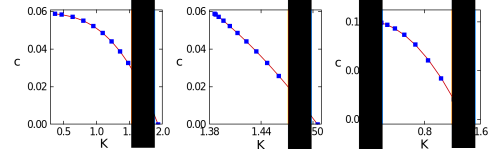
\includegraphics{./../../Graphs/overall-fit.pdf}}
  \caption{The formula (solid lines) giving good approximation to the 
           calculated values (symbols). For the single tip
           calculations, $n=815$ was used, for the double tip $n=995$. 
           $\xi_n = 846$ in both cases.  }\label{fig:overall-fit}
\end{figure}

In all cases, approximate formula can be found for the speed in terms
of the toughness constants. For the single tip case, they are
\begin{equation}
\lambda \approx 0.059 -0.0083 \kappa_I^u + 0.00033 \kappa_I^{3u/2},
\end{equation}
\begin{equation}
\lambda \approx -1.5 +2.7 \kappa_{II} -1.1 \kappa_{II}^2,
\end{equation}
and for the double tip case,
\begin{equation}
\lambda \approx 0.10 - 0.022\kappa_{II}^2.
\end{equation}
These equations provide a fairly good approximation to the data, see figure
\ref{fig:overall-fit}.

In the double tip case, from an energy based theory of fracture mechanics,
one expects a relationship of the form $\lambda = \alpha + \beta 
\kappa_{II}^2$. However, in this case, $\alpha$ and $\beta$ should depend on 
the geometry, $H$, and so should be functions of $\kappa_{II}$. However, 
numerical evidence shows them as being approximately constant. Part of the 
reason for this, is the decoupling between the fluid problem and the dry tip. 
Suppose one solves the two tip problem, for some $L$. This gives a geometry, 
the reference $H'$. From this, one can choose any $\lambda$, and find $G'$, 
and value of $\kappa_{II}$. The effect of this is shown in figure 
\ref{fig:fixed-fluid}, a changing $H'$ has little effect on the $\lambda$, 
$\kappa_{II}$ relationship.


\begin{figure}
 \centerline{
\includegraphics{./../../Graphs/fixed-fluid.pdf}}
  \caption{Reconstructing the full solution given a reference $H'$. Figure 
           made with $n=995$, $\xi_n = 846$.}\label{fig:fixed-fluid}
\end{figure}
\section{Discussion}

Acknowledgements should be included at the end of the paper, before the 
References section or any appendicies, and should be a separate paragraph 
without a heading. Several anonymous individuals are thanked for contributions 
to these instructions.

\bibliographystyle{jfm}
% Note the spaces between the initials
\bibliography{elastic-fracture}

\end{document}
